\documentclass[12pt,a4paper]{article}

\usepackage[margin=2.4cm]{geometry}
\usepackage[T1]{fontenc}
\usepackage[utf8]{inputenc}
\usepackage{array}
\usepackage{booktabs}
\usepackage{longtable}
\usepackage{xcolor}
\usepackage{hyperref}
\usepackage{listings}
\usepackage{tikz}
\usetikzlibrary{arrows.meta,positioning,shapes.geometric,fit}

\definecolor{metablue}{HTML}{1F4E79}
\definecolor{softgray}{HTML}{F4F6F8}
\definecolor{darkgray}{HTML}{333333}
\definecolor{codegray}{HTML}{F7F7F7}
\definecolor{outputgreen}{HTML}{EAF6ED}

\hypersetup{
    colorlinks=true,
    linkcolor=metablue,
    urlcolor=metablue,
    citecolor=metablue
}

\lstdefinelanguage{Go}{
  morekeywords={package,import,func,type,struct,var,const,return,if,else,for,range,defer,go,select,case,default,make,new,nil},
  sensitive=true,
  morecomment=[l]{//},
  morestring=[b]"
}

\lstdefinestyle{code}{
  language=Go,
  basicstyle=\ttfamily\small,
  backgroundcolor=\color{codegray},
  frame=single,
  rulecolor=\color{softgray},
  breaklines=true,
  columns=fullflexible,
  keepspaces=true,
  showstringspaces=false,
  tabsize=2
}

\lstdefinestyle{output}{
  basicstyle=\ttfamily\small,
  backgroundcolor=\color{outputgreen},
  frame=single,
  rulecolor=\color{softgray},
  breaklines=true,
  columns=fullflexible,
  keepspaces=true,
  showstringspaces=false
}

\setlength{\parindent}{0pt}
\setlength{\parskip}{0.75em}
\sloppy

\begin{document}

\begin{titlepage}
    \centering
    {\Large Universita degli Studi di Messina\par}
    \vspace{0.2cm}
    {\large Department of Mathematical, Computer, Physical and Earth Sciences\par}
    \vspace{1.8cm}
    {\Huge\bfseries MetaChat\par}
    \vspace{0.35cm}
    {\LARGE Extended Triple Diffie-Hellman \& Double Ratchet in Go\par}
    \vspace{1.2cm}
    {\large University Project Report\par}
    \vspace{1.5cm}
    \begin{tabular}{rl}
        Creators: & Mehdi Talebikhatir (ID: 558948) \\
                  & Benyamin Baharizadeh (ID: 560587) \\
        Repository: & \url{https://github.com/mehditalebi01/metachat} \\
        Main purpose: & Educational end-to-end encrypted messaging in Go \\
        Date: & April 27, 2026
    \end{tabular}
    \vfill
    {\large Project on secure messaging systems\par}
\end{titlepage}

\tableofcontents
\newpage

\section*{Abstract / Executive Summary}
\addcontentsline{toc}{section}{Abstract / Executive Summary}

MetaChat is a small secure messaging project written in Go. It shows how two users can exchange an encrypted message through a server that does not know the plaintext. The project uses X25519 Diffie-Hellman for shared secret generation, HKDF-SHA256 for key derivation, a Double Ratchet-inspired chain for message keys, AES-256-GCM for authenticated encryption, and Redis as a mailbox for public keys and encrypted messages.

The project is educational. It is close to the ideas used in modern messengers, but it is not a complete production Signal Protocol implementation. In the current code, Benny publishes one X25519 public key, Matteo creates one fresh ephemeral key, both sides derive the same message key, and the server only stores ciphertext. The end-to-end demo was executed successfully: Matteo sent a message, the server queued only encrypted data, and Benny recovered the original text.

\section{Introduction}

Modern messaging applications need more than a password-protected server. A secure messenger should protect the message content even if the server is curious or compromised. This is the main idea of end-to-end encryption: encryption and decryption happen on user devices, while the server is mainly used for delivery.

MetaChat was built to study this idea in a simple way. The repository has three running parts:

\begin{itemize}
    \item \textbf{Benny}: the receiver client, implemented in \texttt{benny/main.go}.
    \item \textbf{Matteo}: the sender client, implemented in \texttt{matteo/main.go}.
    \item \textbf{Relay server}: an HTTP server backed by Redis, implemented in \texttt{server/main.go}.
\end{itemize}

The code also has two internal packages. \texttt{internal/crypto} contains the basic cryptographic operations. \texttt{internal/ratchet} contains the root key, chain key, and message key derivation logic.

\subsection{Project Goal}

The main purpose of this project is to demonstrate an extended Triple Diffie-Hellman and Double Ratchet style secure messaging flow in Go. More specifically, the project shows:

\begin{itemize}
    \item how a receiver can publish a public key before being online;
    \item how a sender can fetch that key and create a shared secret;
    \item how both users can derive the same AES key without sending the key over the network;
    \item how the server can store only public keys, nonces, and ciphertext;
    \item how the receiver can later decrypt the message using its private key.
\end{itemize}

\subsection{Important Scope Note}

The report title uses ``Extended Triple Diffie-Hellman'' because that is the protocol family being studied. The current repository implements a simplified X3DH-inspired handshake. Full X3DH normally uses identity keys, signed prekeys, one-time prekeys, signatures, and identity verification. This project keeps the design smaller so the main learning points are visible in code.

\section{Activities}

The project work can be divided into practical activities. Each activity maps directly to code in the repository.

\begin{longtable}{p{0.24\linewidth} p{0.68\linewidth}}
\toprule
\textbf{Activity} & \textbf{What was done} \\
\midrule
Repository design & The project was split into sender, receiver, server, crypto, and ratchet packages. \\
Key generation & X25519 private and public keys are generated with random 32-byte private keys. \\
Key agreement & Matteo and Benny compute the same shared secret using their own private key and the other side's public key. \\
Key derivation & HKDF-SHA256 is used to derive root keys, chain keys, and one-time message keys. \\
Encryption & AES-256-GCM encrypts the message and authenticates it with a random nonce. \\
Relay server & HTTP endpoints store prekeys and encrypted messages in Redis. \\
End-to-end test & The Go server, Benny client, and Matteo client were executed together and the decrypted output was checked. \\
\bottomrule
\end{longtable}

\section{System Architecture}

The architecture follows a simple client-server-client model. The server is not trusted with plaintext. It is only a relay and storage layer.

\begin{figure}[h]
\centering
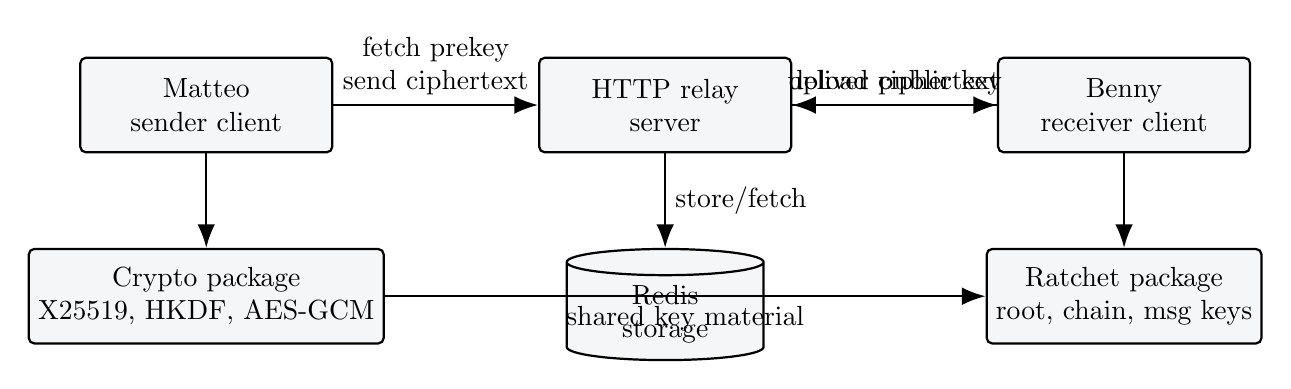
\begin{tikzpicture}[
    node distance=1.4cm,
    box/.style={draw, rounded corners=2pt, thick, align=center, fill=softgray, minimum width=3.2cm, minimum height=1.2cm},
    store/.style={draw, cylinder, shape border rotate=90, aspect=0.25, thick, align=center, fill=softgray, minimum width=2.5cm, minimum height=1.2cm},
    arrow/.style={-{Latex[length=3mm]}, thick}
]
    \node[box] (matteo) {Matteo\\sender client};
    \node[box, right=2.6cm of matteo] (server) {HTTP relay\\server};
    \node[store, below=1.2cm of server] (redis) {Redis\\storage};
    \node[box, right=2.6cm of server] (benny) {Benny\\receiver client};
    \node[box, below=1.2cm of matteo] (crypto) {Crypto package\\X25519, HKDF, AES-GCM};
    \node[box, below=1.2cm of benny] (ratchet) {Ratchet package\\root, chain, msg keys};

    \draw[arrow] (benny) -- node[above, align=center]{upload public key} (server);
    \draw[arrow] (matteo) -- node[above, align=center]{fetch prekey\\send ciphertext} (server);
    \draw[arrow] (server) -- node[right]{store/fetch} (redis);
    \draw[arrow] (server) -- node[above, align=center]{deliver ciphertext} (benny);
    \draw[arrow] (matteo) -- (crypto);
    \draw[arrow] (benny) -- (ratchet);
    \draw[arrow] (crypto) -- node[below, align=center]{shared key material} (ratchet);
\end{tikzpicture}
\caption{MetaChat high-level architecture.}
\end{figure}

\subsection{Main Components}

\begin{longtable}{p{0.22\linewidth} p{0.18\linewidth} p{0.52\linewidth}}
\toprule
\textbf{Component} & \textbf{File} & \textbf{Responsibility} \\
\midrule
Crypto engine & \texttt{internal/crypto/crypto.go} & Generates X25519 keys, computes Diffie-Hellman shared secrets, derives keys with HKDF, encrypts and decrypts with AES-GCM. \\
Ratchet logic & \texttt{internal/ratchet/ratchet.go} & Stores root key and chain key, then advances the chain to produce a new message key. \\
Relay server & \texttt{server/main.go} & Exposes HTTP endpoints and stores data in Redis. It does not decrypt messages. \\
Benny client & \texttt{benny/main.go} & Creates Benny's key pair, uploads the public key, polls the mailbox, derives the key, and decrypts. \\
Matteo client & \texttt{matteo/main.go} & Reads a message, fetches Benny's key, creates an ephemeral key, encrypts, and sends the encrypted message. \\
\bottomrule
\end{longtable}

\section{Protocol Walkthrough}

This section explains the message flow step by step.

\subsection{Step 1: Benny Generates and Publishes a Public Key}

Benny starts first. He creates an X25519 key pair. The private key stays only in Benny's client. The public key is uploaded to the server as a prekey bundle.

\[
\text{Benny key pair} = (bennyPriv, bennyPub)
\]

The server stores the public key under the Redis key:

\begin{lstlisting}[style=output]
prekey:benny
\end{lstlisting}

\subsection{Step 2: Matteo Fetches Benny's Public Key}

Matteo asks the server for Benny's prekey bundle:

\begin{lstlisting}[style=output]
GET /prekey?user=benny
\end{lstlisting}

If Benny has not started yet, the server returns no key and Matteo exits. This is useful in the demo because it makes the correct order clear.

\subsection{Step 3: Matteo Creates a Fresh Ephemeral Key}

Matteo creates a new X25519 key pair only for this message. This limits key reuse.

\[
\text{Matteo ephemeral pair} = (matteoPriv, matteoPub)
\]

The public part is included in the encrypted message object so Benny can compute the same shared secret.

\subsection{Step 4: Both Sides Compute the Same Shared Secret}

Matteo computes:

\[
S = DH(matteoPriv, bennyPub)
\]

Benny later computes:

\[
S = DH(bennyPriv, matteoPub)
\]

Because of the Diffie-Hellman property, both results are the same byte sequence. The server never receives this shared secret.

\subsection{Step 5: The Ratchet Derives the Message Key}

The shared secret is not used directly as an AES key. It is first passed through HKDF and the ratchet:

\begin{lstlisting}[style=output]
root_key  = HKDF(shared_secret, "root")
chain_key = HKDF(root_key, "chain")
chain_key = HKDF(chain_key, "chain-step")
msg_key   = HKDF(chain_key, "msg")
\end{lstlisting}

This gives a 32-byte message key for AES-256-GCM.

\subsection{Step 6: Matteo Encrypts and Sends}

Matteo encrypts the plaintext with AES-GCM. The server receives this object:

\begin{lstlisting}[style=code, caption={Secure message format from server/main.go}]
type SecureMessage struct {
    FromIdentity []byte `json:"from_identity"`
    EphemeralKey []byte `json:"ephemeral_key"`
    Nonce        []byte `json:"nonce"`
    Ciphertext   []byte `json:"ciphertext"`
}
\end{lstlisting}

The server stores it in:

\begin{lstlisting}[style=output]
secure_mailbox:benny
\end{lstlisting}

\subsection{Step 7: Benny Fetches and Decrypts}

Benny polls his mailbox. When a message exists, he uses Matteo's ephemeral public key and his own private key to derive the same message key. Then AES-GCM opens the ciphertext and returns the plaintext.

\section{Real Code Evidence}

This section includes real parts of the repository code. The snippets are shortened only to keep the report readable.

\subsection{Key Generation and Diffie-Hellman}

\begin{lstlisting}[style=code, caption={X25519 key generation and shared secret in internal/crypto/crypto.go}]
func GenerateKeyPair() (priv, pub []byte) {
    priv = make([]byte, 32)
    rand.Read(priv)
    pub, _ = curve25519.X25519(priv, curve25519.Basepoint)
    return
}

func DH(priv, pub []byte) []byte {
    shared, _ := curve25519.X25519(priv, pub)
    return shared
}
\end{lstlisting}

This is the base of the key exchange. Each side uses a private key and the other side's public key. The result becomes the input to the key derivation process.

\subsection{HKDF and AES-GCM}

\begin{lstlisting}[style=code, caption={HKDF and AES-GCM helpers in internal/crypto/crypto.go}]
func HKDF(secret []byte, info string) []byte {
    h := hkdf.New(sha256.New, secret, nil, []byte(info))
    out := make([]byte, 32)
    io.ReadFull(h, out)
    return out
}

func Encrypt(key, plaintext []byte) (nonce, ciphertext []byte) {
    block, _ := aes.NewCipher(key)
    gcm, _ := cipher.NewGCM(block)
    nonce = make([]byte, gcm.NonceSize())
    rand.Read(nonce)
    ciphertext = gcm.Seal(nil, nonce, plaintext, nil)
    return
}
\end{lstlisting}

HKDF separates different key uses through the \texttt{info} string. AES-GCM gives confidentiality and integrity: if the ciphertext or tag is changed, decryption should fail.

\subsection{Ratchet Chain}

\begin{lstlisting}[style=code, caption={Message key derivation in internal/ratchet/ratchet.go}]
func NewRatchet(sharedSecret, remotePub []byte) *Ratchet {
    priv, pub := crypto.GenerateKeyPair()
    root := crypto.HKDF(sharedSecret, "root")
    chain := crypto.HKDF(root, "chain")
    return &Ratchet{
        RootKey:   root,
        ChainKey:  chain,
        DHPriv:    priv,
        DHPub:     pub,
        RemotePub: remotePub,
    }
}

func (r *Ratchet) NextMessageKey() []byte {
    r.ChainKey = crypto.HKDF(r.ChainKey, "chain-step")
    return crypto.HKDF(r.ChainKey, "msg")
}
\end{lstlisting}

The chain key moves forward before a message key is created. In a larger implementation, this would be repeated for every message.

\subsection{Server Endpoints}

\begin{lstlisting}[style=code, caption={HTTP route setup in server/main.go}]
http.HandleFunc("/upload_prekey", uploadPrekey)
http.HandleFunc("/prekey", getPrekey)
http.HandleFunc("/send_secure", sendSecure)
http.HandleFunc("/fetch_secure", fetchSecure)
\end{lstlisting}

The endpoints are deliberately simple. The server stores a public key and a ciphertext mailbox. It has no code path that uses AES or reads plaintext.

\subsection{Matteo Sender Flow}

\begin{lstlisting}[style=code, caption={Matteo derives a key and encrypts in matteo/main.go}]
matteoPriv, matteoPub := crypto.GenerateKeyPair()

shared := crypto.DH(matteoPriv, bundle.IdentityKey)
r := ratchet.NewRatchet(shared, bundle.IdentityKey)
msgKey := r.NextMessageKey()

nonce, ciphertext := crypto.Encrypt(msgKey, []byte(message))

msg := SecureMessage{
    FromIdentity: matteoPub,
    EphemeralKey: matteoPub,
    Nonce:        nonce,
    Ciphertext:   ciphertext,
}
\end{lstlisting}

\subsection{Benny Receiver Flow}

\begin{lstlisting}[style=code, caption={Benny derives the same key and decrypts in benny/main.go}]
shared := crypto.DH(bennyPriv, msg.EphemeralKey)
r := ratchet.NewRatchet(shared, msg.EphemeralKey)
msgKey := r.NextMessageKey()

plaintext := crypto.Decrypt(msgKey, msg.Nonce, msg.Ciphertext)
fmt.Println("[BENNY] Benny received:", string(plaintext))
\end{lstlisting}

This proves the important protocol point: Matteo and Benny do not exchange the AES key. They calculate it independently.

\section{Results \& Discussion}

\subsection{Build and Package Check}

The Go packages were checked with \texttt{go test ./...}. A local build cache was used because the default Windows Go cache was not writable in this environment.

\begin{lstlisting}[style=output, caption={Go package check output}]
?       metachat/benny              [no test files]
?       metachat/internal/crypto    [no test files]
?       metachat/internal/ratchet   [no test files]
?       metachat/matteo             [no test files]
?       metachat/server             [no test files]
\end{lstlisting}

This means all packages compiled successfully. The project does not currently include automated unit tests.

\subsection{End-to-End Demo Output}

The real Go server and clients were executed. Redis was not installed on the machine, so the demo used a small local Redis-compatible test relay that supported only the Redis commands used by this project: \texttt{PING}, \texttt{SET}, \texttt{GET}, \texttt{LPUSH}, and \texttt{RPOP}. The Go code itself was not changed.

\begin{lstlisting}[style=output, caption={Server output}]
[SERVER] Running on :8080 (Redis: localhost:6379)
[SERVER] Stored prekey bundle for benny (Redis key: prekey:benny)
[SERVER] Served prekey bundle for benny
[SERVER] Queued secure message for benny (Redis list: secure_mailbox:benny)
[SERVER] Delivered 1 secure message to benny
\end{lstlisting}

\begin{lstlisting}[style=output, caption={Matteo output}]
[MATTEO] Message from CLI args: Hello Benny, this is a secure MetaChat demo for the university report.
[MATTEO] Fetching Benny prekey from server...
[MATTEO] Benny prekey received.
[MATTEO] Generating Matteo ephemeral X25519 keypair...
[MATTEO] Computing shared secret (X25519 DH)...
[MATTEO] Initializing ratchet and deriving message key...
[MATTEO] Encrypting message with AES-GCM...
[MATTEO] Sending encrypted message to server (queued for benny in Redis)...
[MATTEO] Done. Message sent.
\end{lstlisting}

\begin{lstlisting}[style=output, caption={Benny output}]
[BENNY] Generating Benny X25519 identity keypair...
[BENNY] Uploading Benny public key to server (stored in Redis as prekey:benny)...
[BENNY] Benny ready. Polling mailbox from server (secure_mailbox:benny in Redis)...
[BENNY] Received encrypted message. Deriving shared secret (X25519 DH)...
[BENNY] Initializing ratchet and deriving message key...
[BENNY] Decrypting with AES-GCM...
[BENNY] Benny received: Hello Benny, this is a secure MetaChat demo for the university report.
\end{lstlisting}

The result is correct. The plaintext appears only in Matteo's local input and Benny's final output. The server output only shows storage and delivery actions.

\subsection{What Worked Well}

\begin{itemize}
    \item The project has a clean separation between crypto logic, ratchet logic, clients, and server.
    \item The server does not need private keys or plaintext to deliver the message.
    \item X25519 keeps the key exchange simple and modern.
    \item AES-GCM provides both encryption and tamper detection.
    \item Redis lists are a good fit for a simple asynchronous mailbox.
\end{itemize}

\subsection{Security Limitations}

The current version is a good lab project, but it should not be used as a real secure messenger yet.

\begin{longtable}{p{0.28\linewidth} p{0.62\linewidth}}
\toprule
\textbf{Limitation} & \textbf{Explanation} \\
\midrule
Simplified X3DH & The code uses one published receiver public key and one sender ephemeral key. It does not yet include signed prekeys, one-time prekeys, signatures, or identity verification. \\
Partial Double Ratchet & The code derives chain keys and message keys, but the full send/receive Double Ratchet state, skipped message keys, and out-of-order handling are not implemented. \\
No identity verification & Users do not compare safety numbers, fingerprints, or QR codes. A malicious server could replace a public key. \\
No replay protection & There are no message counters or message IDs to detect repeated ciphertext. \\
No transport TLS & The demo uses plain HTTP to the relay server. The message content is still encrypted, but metadata and requests are visible on the network. \\
Error handling in crypto & Some errors from \texttt{rand.Read}, \texttt{curve25519.X25519}, and AES-GCM open are ignored. Production code should return and check these errors. \\
Key persistence & Keys are generated each run and are not stored securely for longer conversations. \\
\bottomrule
\end{longtable}

\subsection{Suggested Future Work}

\begin{itemize}
    \item Add a complete X3DH prekey bundle: identity key, signed prekey, signed prekey signature, and one-time prekeys.
    \item Add identity verification with fingerprints or QR codes.
    \item Implement full Double Ratchet state for both directions, including message counters and skipped message keys.
    \item Use associated data in AES-GCM to bind metadata such as sender, receiver, and message number.
    \item Add TLS for client-server traffic.
    \item Return errors from crypto functions instead of ignoring them.
    \item Add unit tests for key agreement, ratchet key equality, encryption, failed decryption, and server handlers.
\end{itemize}

\section{Conclusion}

MetaChat successfully demonstrates the core idea of an end-to-end encrypted messenger. The server helps users find keys and deliver messages, but it does not decrypt the message. Matteo and Benny independently derive the same message key using X25519 and HKDF, then AES-GCM protects the message content.

The project is valuable because the implementation is small enough to study line by line. It shows why modern secure messengers use a mix of public-key agreement, symmetric encryption, key derivation, ratcheting, and server-side queues. The main improvement needed is to move from a simplified educational protocol toward a complete X3DH and Double Ratchet implementation with identity verification, replay protection, and stronger error handling.

\appendix

\section{Appendix A: Modern Messengers Today}

Most current secure messengers use a similar split between delivery and confidentiality. The server handles accounts, routing, push notifications, and storage of encrypted messages. The clients handle keys, encryption, and decryption.

Signal's public specifications describe X3DH as a protocol for asynchronous key agreement, where one user can publish prekeys to a server and another user can start an encrypted session while the first user is offline. Signal's Double Ratchet specification describes the use of KDF chains, a symmetric-key ratchet, and a Diffie-Hellman ratchet for fresh message keys.

WhatsApp and Messenger also use Signal Protocol ideas for end-to-end encrypted personal communication. Meta has also published work on key transparency, which helps users check that a public key directory has not secretly been changed.

Telegram is different: normal cloud chats are server-synced, while Secret Chats are the end-to-end encrypted mode. Telegram's own documentation says Secret Chats use keys held only by the participants and are device-specific.

MetaChat is not as complete as these systems, but it is a useful small version of the same design pattern:

\begin{itemize}
    \item public keys are published before communication;
    \item a server relays messages but should not know plaintext;
    \item clients derive symmetric message keys;
    \item message keys should change over time.
\end{itemize}

\section{Appendix B: API Endpoints}

\begin{longtable}{p{0.14\linewidth} p{0.24\linewidth} p{0.18\linewidth} p{0.34\linewidth}}
\toprule
\textbf{Method} & \textbf{Endpoint} & \textbf{Query} & \textbf{Purpose} \\
\midrule
POST & \texttt{/upload\_prekey} & \texttt{user} & Upload a user's public key bundle. \\
GET & \texttt{/prekey} & \texttt{user} & Fetch a user's public key bundle. \\
POST & \texttt{/send\_secure} & \texttt{to} & Queue an encrypted message for a receiver. \\
GET & \texttt{/fetch\_secure} & \texttt{user} & Pop the next encrypted message from a mailbox. \\
\bottomrule
\end{longtable}

\section{Appendix C: Redis Keys}

\begin{longtable}{p{0.32\linewidth} p{0.16\linewidth} p{0.42\linewidth}}
\toprule
\textbf{Redis key} & \textbf{Type} & \textbf{Meaning} \\
\midrule
\texttt{prekey:<user>} & String & JSON-encoded public key bundle. \\
\texttt{secure\_mailbox:<user>} & List & Queue of encrypted messages waiting for the user. \\
\bottomrule
\end{longtable}

\section{Appendix D: Repository Structure}

\begin{lstlisting}[style=output]
metachat/
  go.mod
  README.md
  securechat.pdf
  server/main.go
  matteo/main.go
  benny/main.go
  internal/crypto/crypto.go
  internal/ratchet/ratchet.go
\end{lstlisting}

\section{References}

\begin{enumerate}
    \item Signal, ``The X3DH Key Agreement Protocol.'' \url{https://signal.org/docs/specifications/x3dh/}
    \item Signal, ``The Double Ratchet Algorithm.'' \url{https://signal.org/docs/specifications/doubleratchet/}
    \item Meta Engineering, ``Deploying key transparency at WhatsApp.'' \url{https://engineering.fb.com/2023/04/13/security/whatsapp-key-transparency/}
    \item Telegram, ``End-to-End Encryption, Secret Chats.'' \url{https://core.telegram.org/api/end-to-end}
    \item Go package documentation, \texttt{golang.org/x/crypto/curve25519}. \url{https://pkg.go.dev/golang.org/x/crypto/curve25519}
\end{enumerate}

\end{document}
